\begin{frame}
    \frametitle{Научная новизна}
    \begin{itemize}
        \item Разработанный метод обучения с подкреплением, способный оперировать действиями различного масштаба и устойчивый к оптическим шумам, впервые был применен для настройки оптического интерферометра.
        \item Впервые создан программно-аппаратный комплекс настройки оптического интерферометра по изображениям с камеры, основанный на машинном обучении с подкреплением.
        \item Был разработан метод, позволяющий достичь сходимости к хорошему оптимутму для многозадачного агента. Разработанный метод был применен для управления движением шагающего робота с заданной линейной и угловой скоростью.
        \item Была предложена идея иерархического алгоритма, сочетающего в себе машинное обучения с подкреплением и запрограммированное поведение. 
        Разработанный алгоритм был применен для управления агентом в игре NetHack. 
    \end{itemize}
\end{frame}
\note{
    Проговаривается вслух научная новизна
}

\begin{frame}
    \frametitle{Научная и практическая значимость}
    \begin{itemize}
        \item Применение предложенного в работе автоматизированного подхода к настройке оптического интерферометра позволит существенно ускорить проведение физических экспериментов и снизит необходимость в ручном труде.
        \item Разработанные алгоритмы для управления виртуальными агентами затем могут быть применены в робототехнике, самоуправляемых автомобилях и виртуальных ассистентах.
    \end{itemize}
\end{frame}
\note{
    Проговариваются вслух научная и практическая значимость
}

\begin{frame}
    \frametitle{Свидетельство о регистрации программы}
    \begin{figure}[h]
        \centering
        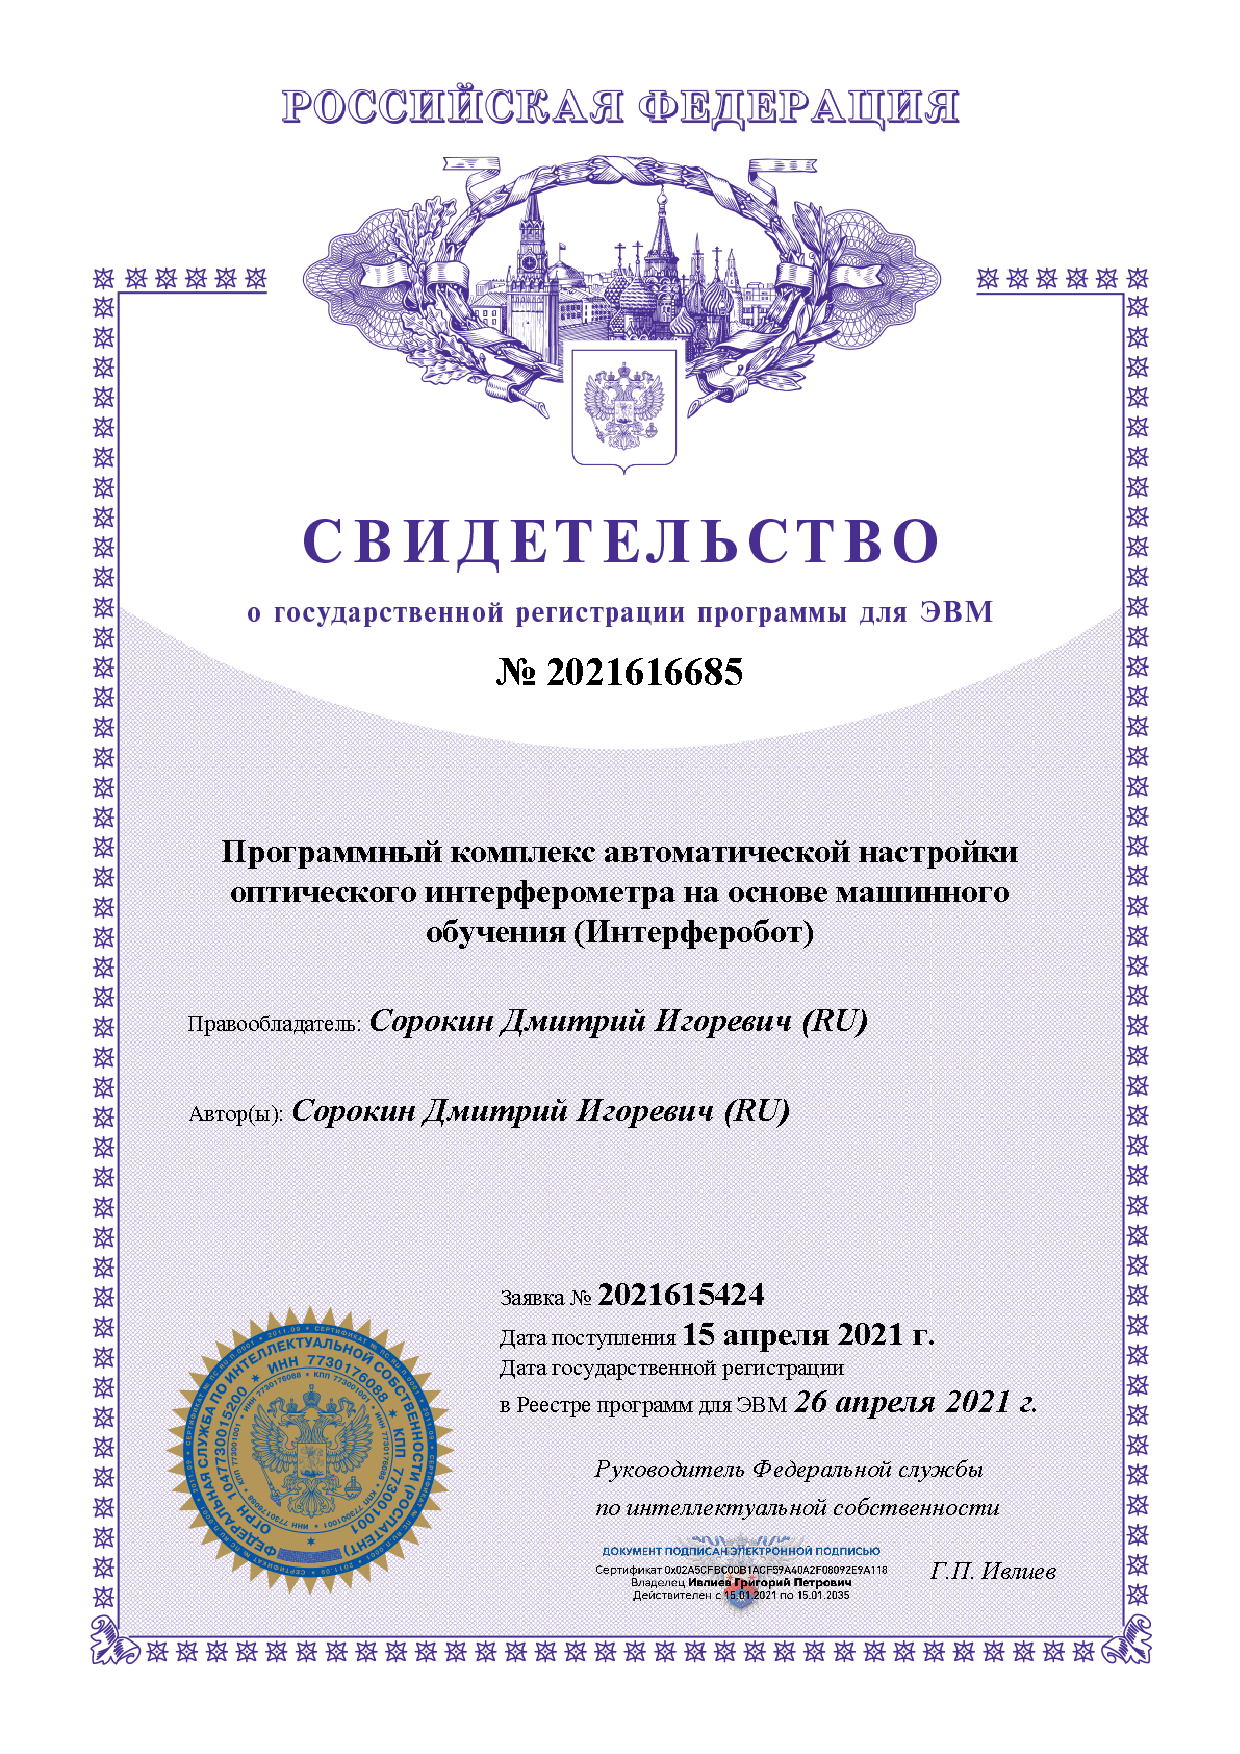
\includegraphics[height=0.7\textheight]{interferobot_rid.pdf}
    \end{figure}
\end{frame}
\note{
    Получено свидетельство о регистрации разработанной программы \textsc{Hello~world™}.
}

%\begin{frame}
%    \frametitle{Акт о внедрении}
%    \begin{figure}[h]
%        \centering
%        \fbox{
%            \begin{minipage}[t]{0.4\linewidth}
%                %\includegraphics[width=\linewidth]{implementation}
%            \end{minipage}
%        }
%    \end{figure}
%\end{frame}
%\note{
%    Получен акт о внедрении.
%}

%\begin{frame} % публикации на одной странице
\begin{frame}[t,allowframebreaks] % публикации на нескольких страницах
\frametitle{Публикации результатов диссертационной работы}

\begin{enumerate}
\fontsize{10pt}{10pt}\selectfont
    \item Interferobot: aligning an optical interferometer by a reinforcement learning agent. \textcolor{gray}{/. –– }\textbf{D. Sorokin}\textcolor{gray}{, A. Ulanov, E. Sazhina, A. Lvovsky // Advances in Neural Information Processing Systems. Vol. 33 / ed. by H. Larochelle, M. Ranzato, R. Hadsell, M. F. Balcan, H. Lin. –– Curran Associates, Inc., 2020. –– P. 13238––13248.} (CORE A*)
    \item Aligning an optical interferometer with beam divergence control and continuous action space. \textcolor{gray}{/. –– S. Makarenko,} \textbf{D. I. Sorokin}\textcolor{gray}{, A. Ulanov, A. Lvovsky // Proceedings of the 5th Conference on Robot Learning. Vol. 164 / ed. by A. Faust, D. Hsu, G. Neumann. –– PMLR, 2022. –– P. 918––927. –– (Proceedings of Machine Learning Research)}
    \item Insights From the NeurIPS 2021 NetHack Challenge. \textcolor{gray}{/. –– E. Hambro, S. Mohanty, D. Babaev, M. Byeon, D. Chakraborty, E. Grefenstette, M. Jiang, J. Daejin, A. Kanervisto, J. Kim, S. Kim, R. Kirk, V. Kurin, H. Küttler, T. Kwon, D. Lee, V. Mella, N. Nardelli, I. Nazarov, N. Ovsov, J. Holder, R. Raileanu, K. Ramanauskas, T. Rocktäschel, D. Rothermel, M. Samvelyan,} \textbf{D. Sorokin}\textcolor{gray}{, M. Sypetkowski, M. Sypetkowski // Proceedings of the NeurIPS 2021 Competitions and Demonstrations Track. Vol. 176 / ed. by D. Kiela, M. Ciccone, B. Caputo. –– PMLR, 2022. –– P. 41––52. –– (Proceedings of Machine Learning Research)} (CORE A*)
    \item Learning Various Locomotion Skills from Scratch with Deep Reinforcement Learning. \textcolor{gray}{/. –– }\textbf{D. I. Sorokin}\textcolor{gray}{, D. L. Babaev // Advances in Neural Computation, Machine Learning, and Cognitive Research VI / ed. by B. Kryzhanovsky, W. Dunin-Barkowski, V. Redko, Y. Tiumentsev. –– Cham : Springer International Publishing, 2023. –– P. 322––329.} (SCOPUS)
\end{enumerate}
    
\end{frame}
\note{
    Результаты работы опубликованы в N печатных изданиях,
    в~т.\:ч. M реферируемых изданиях.
}

\begin{frame}
    \frametitle{Участие в конференциях}
    \begin{itemize}
        \item 34 международная конференции Neural Information Processing Systems (NeurIPS 2020) (доклад был отмечен как spotlight).
        \item 29 международная конференция по лазерной физике LPHYS’21
        \item 5 международная конференция Conference on Robot Learning (CoRL 2021).
        \item  35 международная конференция Neural Information Processing Systems (NeurIPS, Competition track 2021).
        \item Международная конференция по квантовым технологиям ICQT 2021.
        \item Международная научно-техническая конференция Нейроинформатика 2022.
    \end{itemize}
\end{frame}
\note{
    Работа была представлена на ряде конференций.
}

\begin{frame}[plain, noframenumbering] % последний слайд без оформления
    \begin{center}
        \Huge
        Спасибо за внимание!
    \end{center}
\end{frame}
